\documentclass[12pt]{article}
\usepackage[top=1in,left=1in, right = 1in, footskip=1in]{geometry}

\usepackage{graphicx}
%\usepackage{adjustbox}

%% \newcommand{\comment}{\showcomment}
\newcommand{\comment}{\nocomment}

\newcommand{\showcomment}[3]{\textcolor{#1}{\textbf{[#2: }\textsl{#3}\textbf{]}}}
\newcommand{\nocomment}[3]{}

\newcommand{\jd}[1]{\comment{cyan}{JD}{#1}}
\newcommand{\swp}[1]{\comment{magenta}{SWP}{#1}}

\newcommand{\eref}[1]{(Eq.~\ref{eq:#1})}
\newcommand{\fref}[1]{Fig.~\ref{fig:#1}}
\newcommand{\Fref}[1]{Fig.~\ref{fig:#1}}
\newcommand{\sref}[1]{Sec.~\ref{#1}}
\newcommand{\frange}[2]{Fig.~\ref{fig:#1}--\ref{fig:#2}}
\newcommand{\tref}[1]{Table~\ref{tab:#1}}
\newcommand{\tlab}[1]{\label{tab:#1}}
\newcommand{\seminar}{SE\mbox{$^m$}I\mbox{$^n$}R}

\usepackage{amsthm}
\usepackage{amsmath}
\usepackage{amssymb}
\usepackage{amsfonts}

% \usepackage{lineno}
% \linenumbers

\usepackage[pdfencoding=auto, psdextra]{hyperref}

\usepackage[numbers]{natbib}
\usepackage{hyperref,url}
\bibliographystyle{unsrt}
\date{\today}

\usepackage{xspace}
\newcommand*{\ie}{i.e.\@\xspace}

\usepackage{color}

\newcommand{\Rx}[1]{\ensuremath{{\mathcal R}_{#1}}} 
\newcommand{\Ro}{\Rx{0}}
\newcommand{\RR}{\ensuremath{{\mathcal R}}}
\newcommand{\Rhat}{\ensuremath{{\hat\RR}}}
\newcommand{\tsub}[2]{#1_{{\textrm{\tiny #2}}}}

\begin{document}

\begin{flushleft}{
	\Large
	\textbf\newline{
		Potential roles of social distancing in preventing the spread of coronavirus disease 2019 (COVID-19) in South Korea
	}
}
\newline
\\
Sang Woo Park\textsuperscript{1,*}
Kaiyuan Sun\textsuperscript{2}
C\'ecile Viboud\textsuperscript{2}
Jonathan Dushoff\textsuperscript{3,4,5}
Bryan T.\ Grenfell\textsuperscript{1,2,6}
\\
\bigskip
\textbf{1} Department of Ecology and Evolutionary Biology, Princeton University, Princeton, NJ, USA
\\
\textbf{2} Fogarty International Center, National Institutes of Health, Bethesda, MD, USA
\\
\textbf{3} Department of Mathematics and Statistics, McMaster University, Hamilton, ON, Canada
\\
\textbf{4} M.\,G.\,DeGroote Institute for Infectious Disease Research, McMaster University, Hamilton, ON, Canada
\\
\textbf{5} Department of Biology, McMaster University, Hamilton, ON, Canada
\\
\textbf{6} Woodrow Wilson School of Public and International Affairs, Princeton University, Princeton, NJ, USA
\\
\bigskip

*Corresponding author: swp2@princeton.edu
\end{flushleft}

\pagebreak

Since its first appearance in Wuhan, China, in December 2019, the novel coronavirus disease (COVID-19) has spread internationally, including to South Korea.
The first COVID-19 case in South Korea was confirmed on January 20, 2020, from a traveling resident of Wuhan, China \citep{kcdc}.
The epidemic then took off in mid-February when COVID-19 began to spread within a church from a city of Daegu --- as of March 18, 2020, 8,413 cases have been confirmed, of which 60\% are related to the church \citep{kcdc}.
While its success in controlling the epidemic has been widely attributed to its extensive testing \citep{science}, other factors, such as social distancing, are also likely to have played important roles.
Here, we compare epidemics in two geographically separated major cities in South Korea and use traffic data to study potential roles of social distancing in mitigating the spread of COVID-19.

\section{Data description}

We analyze epidemiological data, collected bewteen January 20--March 16, 2020, describing the COVID-19 outbreak in Korea.
Daily number of reported cases in each geographic region was transcribed from press releases by Korea Centers for Disease Control and Prevention (KCDC) \cite{kcdc}.
Partial line lists were transcribed from press releases and reports from KCDC and various local and provincial government websites.
All data and original reports are stored in a publicly available GitHub repoository: \url{https://github.com/parksw3/COVID19-Korea}.

\begin{figure}[!h]
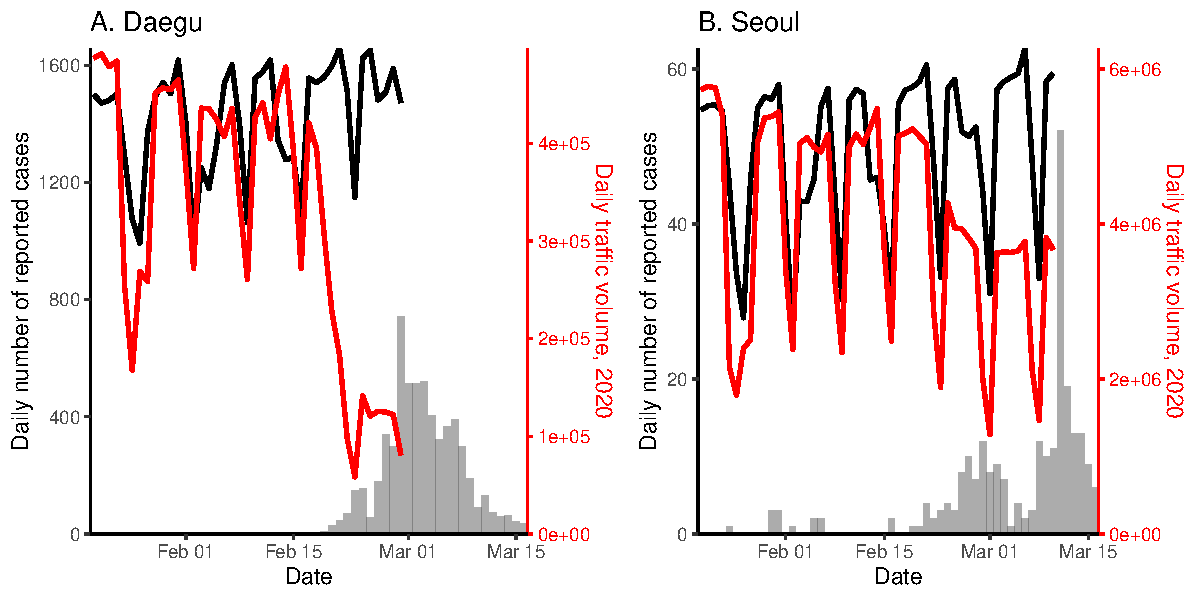
\includegraphics[width=\textwidth]{figure_compare_report.pdf}
\caption{
\textbf{Comparison of epidemiological and traffic data from Daegu and Seoul.}
Red lines represent the daily metro traffic volume in 2020.
Black lines represent the average daily metro traffic volume in previous years, 2017--2019.
Daily traffic from previous years have been shifted by 1--3 days to align day of the week.
Vertical lines indicate Feb 18, 2020, when the first case was confirmed in Daegu.
}
\label{fig:data}
\end{figure}

We compare epidemiological dynamics of COVID-19 from two cities in which the biggest number of COVID-19 cases have been reported: Daegu and Seoul.
Bewteen January 20--March 16, 2020, 6,083 cases were reported from Daegu and 248 from Seoul.
Unlike the epidemic in Daegu, which is characterized by a single, large peak followed by a gradual decrease in the number of confirmed cases, the epidemic in Seoul consists of several small outbreaks (\fref{data}).

Daily metro traffic in Daegu and Seoul between 2017--2020 was obtained from \url{data.go.kr} and \url{data.seoul.go.kr}.
\fref{data} compares the daily number of individuals who got on the subway --- including a monorail in Daegu --- across all stations.
Soon after the first church-related case was confirmed in Daegu on Feb 18, 2020, the daily traffic volume decreased by about 80\% and 50\% compared to previous years in Daegu and Seoul, respectively.

%% https://www.data.go.kr/dataset/15002503/fileData.do
%% https://data.seoul.go.kr/dataList/OA-12914/S/1/datasetView.do

\section{Trends in time-dependent reproduction number and traffic volume}

We estimate the time-dependent reproduction number $R_t$ (i.e., the expected number of secondary cases caused by an individual infected at time $t$ \citep{fraser2007estimating}) for both epidemics.
We account for changes in testing criteria, which occurred 5 times, by multiplying the number of positive cases by their relative detection rate (i.e., a proportion of cases tested positive based on a criterion divided by the mean detection rate).
Likewise, we account for changes in the number of tests completed on each day by dividing the number of positive cases again by the relative number of tests completed on each day; this step is performed separately for each testing criterion because the widening of a criterion necessarily increases the number of tests.
A sensitivity analysis showed that qualitative patterns of inferred $R_t$ are robust to these adjustments (Supplementary Materials).

We estimate the time-varying \emph{backward} confirmation-to-onset delay distributions from the partial line list and combine them with previously estimated incubation period distribution \citep{backer2020incubation} to infer the probability distributions for date of infection of each confirmed case.
To account for right-censoring (i.e., individuals that are infected but have not been confirmed yet), we estimate the time-varying \emph{forward} onset-to-confirmation delay distribution, and infer the probability that a case infected on a given day will be reported before March 16, 2020.
Then, we divide the reconstructed incidence time series (i.e., the number of infected individuals on day $t$) by this probability and estimate the time-dependent reproduction number using the renewal equation using a 14-day sliding window \citep{fraser2007estimating}:
\begin{equation}
\mathcal R_t = \frac{I_t}{\sum_{k=1}^{14} I_{t-k} w_k},
\end{equation}
where $I_t$ is the censoring-adjusted incidence time series and $w_k$ is the generation-interval distribution.
We only calculate the time-dependent reproduction number until March 10, 2020 because the degree of right-censoring too large afterwards.
Details are provided in the Supplementary Materials.

\begin{figure}[!ht]
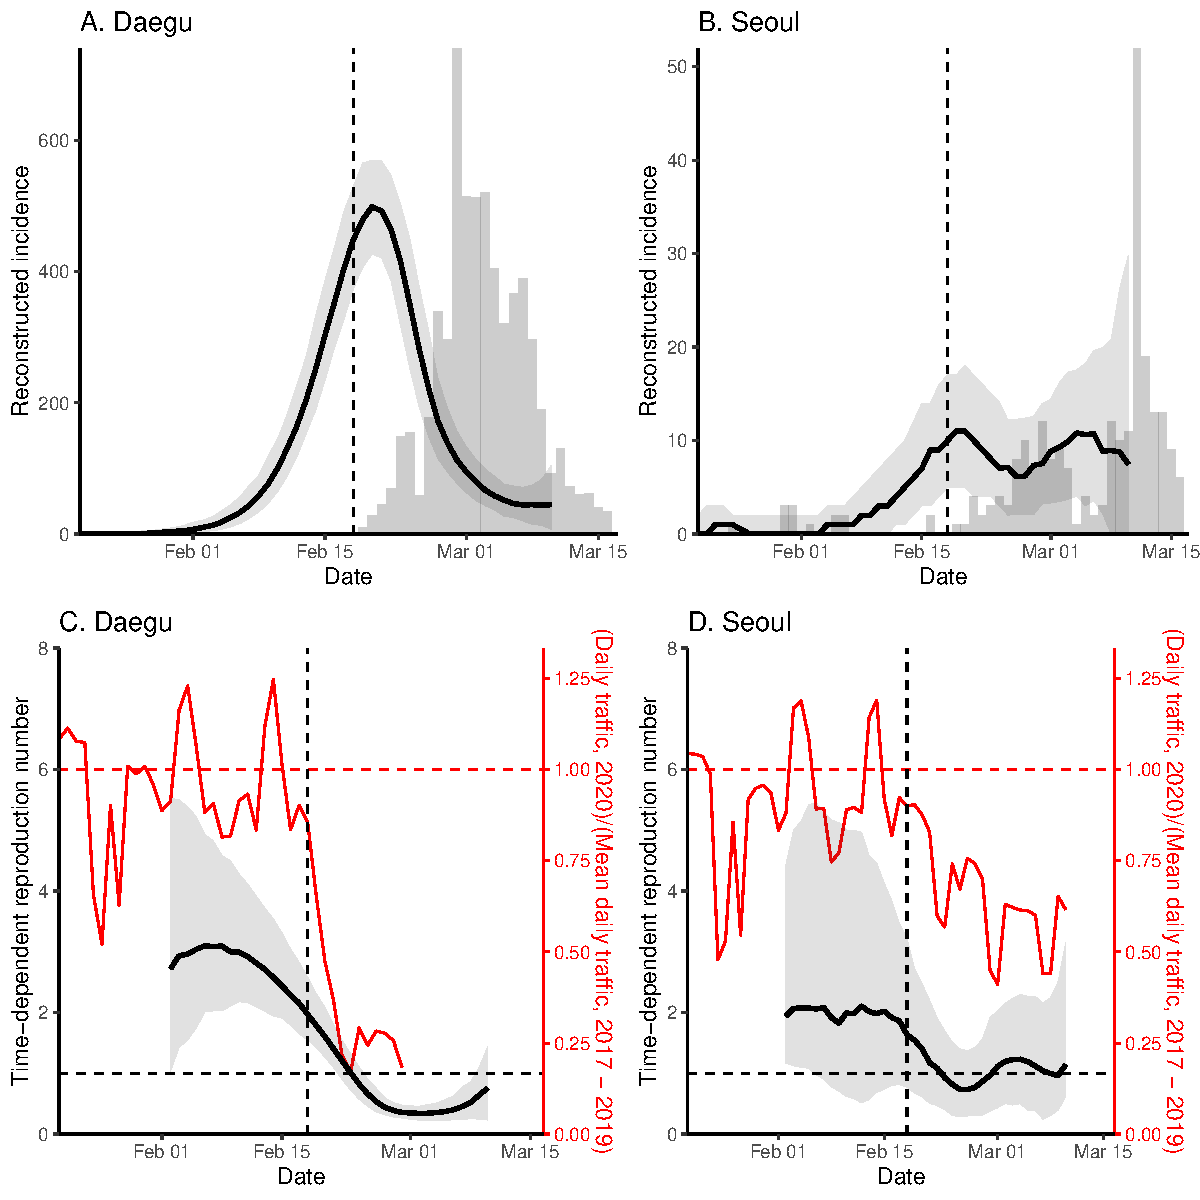
\includegraphics[width=\textwidth]{figure_compare_R_t.pdf}
\caption{
\textbf{Comparison of time-dependent reproduction number and normalized traffic in Daegu and Seoul.}
Black lines represent the median estimates of $R_t$. 
Gray ribbons represent the corresponding 95\% credible intervals.
Red lines represent the normalized traffic volume.
Vertical lines indicate Feb 18, 2020, when the first case was confirmed in Daegu.
}
\label{fig:eff}
\end{figure}

\fref{eff} compares the estimates of $\mathcal R_t$ in Daegu and Seoul.
Estimates of $\mathcal R_t$ gradually decrease in Daegu and eventually drop below 1 about a week after the introduction of its first case, coinciding with the decrease in the metro traffic volume (\fref{eff}A);
our estimates of $\mathcal R_t$ are consistent with \cite{tempvar}, although their $\mathcal R_t$ estimates drop below 1 slightly later because they rely on number of symptomatic cases instead.
On the other hand, estimates of $\mathcal R_t$ remain around 1 in Seoul (\fref{eff}B), suggesting that the degree of social distancing may have been insufficient to prevent the spread in Seoul;
stronger distancing or other control measures will be required to decrease $\mathcal R_t$ below 1.
Similar patterns in the estimates of $\mathcal R_t$ are found in adjacent provinces, providing support for the robustness of our analysis (Supplementary Materials).

\section{Discussion}

The ongoing COVID-19 outbreak in South Korea provides a unique perspective to understanding and controlling the pandemic.
Its experience provides evidence that the epidemic can be contained without draconian measures as in China.
Our analysis provides indirect, but clear, evidence that social distancing is likely to have assisted in mitigating the epidemic in South Korea.
Even though social distancing alone may not be able to fully prevent the spread of the disease, its ability to flatten the epidemic curve (cf. \fref{eff}B) reduces burden for healthcare system and provides time to plan for the future \citep{anderson2020will}.

There are several limitations to our study.

Finally, while there is a clear 

Caveats:
\begin{itemize}
  \item Only two cities...although two coupled provinces show strikingly similar patterns
  \item Correlation not causation
  \item Did not account for geographic heterogeneity in testing or etc. Estimation of delay distribution etc all based on national line list.
\end{itemize}

\section*{Contribution}

Data collection: SWP; conceptualisation: SWP and CV; analysis: SWP; first draft: SWP, JD. All authors contributed to the writing and approval of the final report.

\pagebreak

\bibliography{korea}

\section{Supplementary Materials}

\begin{figure}[!ht]
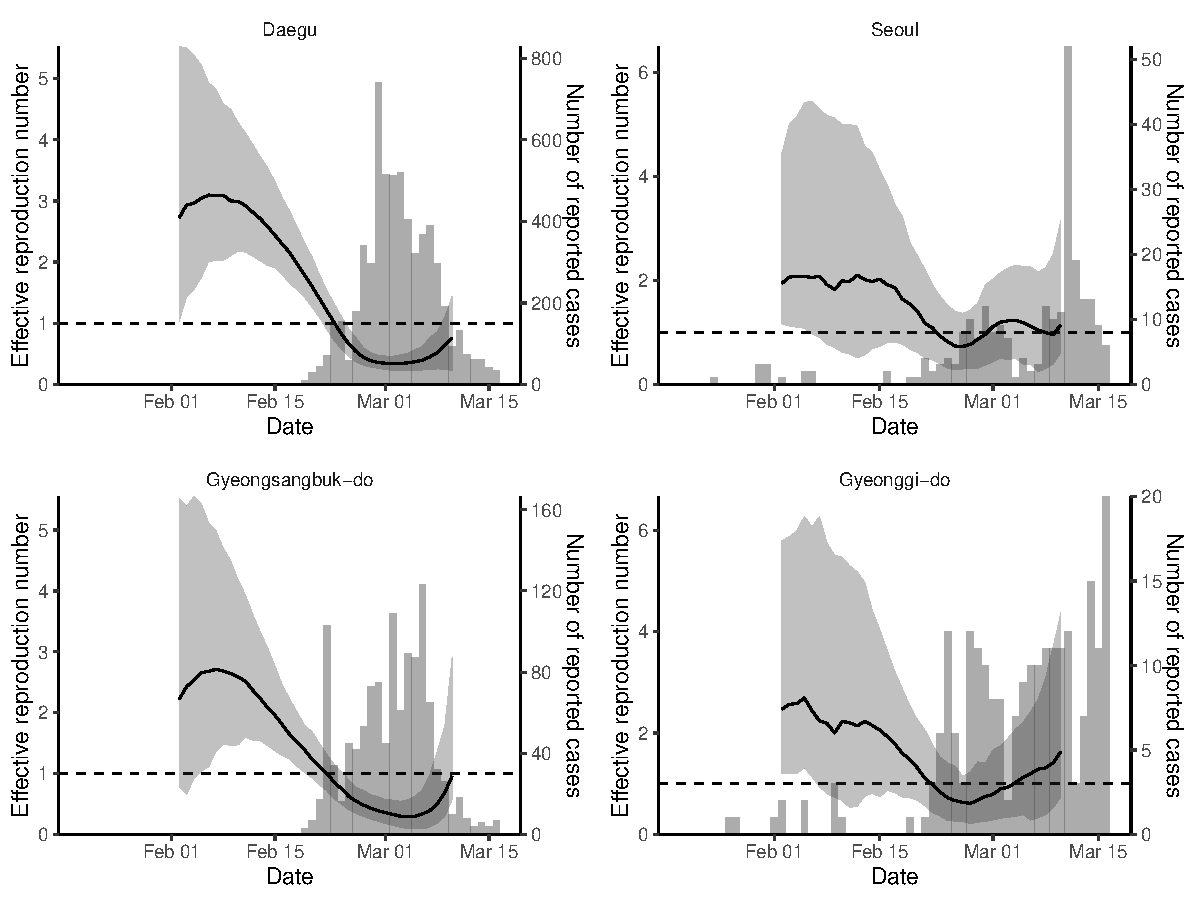
\includegraphics[width=\textwidth]{figure_R_t_all.pdf}
\caption{
\textbf{Comparison of effective reproduction number in Daegu, Seoul, Gyeongsangbuk-do, and Gyeonggi-do.}
}
\end{figure}

\end{document}
